\section{Manual de Uso}

\subsection{Formato del Archivo}

\javapetriconcurrencymonitor utiliza el formato estándar PNML para descripción
de redes de Petri, específicamente el dialecto del editor TINA\cite{TinaSite}.

Para más información sobre el estándar PNML, el sitio online de referencia del
lenguaje es \cite{PnmlSite}.

\begin{framed}
\paragraph{Nota:}
Como TINA no tiene soporte para arcos de reset, el usuario debe especificar
este tipo de conexión modificando el archivo PNML con un editor de texto.
Se recomienda utilizar otro tipo de arco en TINA y luego cambiar el valor del
campo \textit{``type''} del arco correspondiente en el archivo PNML.

Ej:
\begin{figure}[H]
\centering
\begin{minted}{xml}
<arc id="e-1" source="p-1" target="t-1">
  <type value="reset"/>
</arc>
\end{minted}
\end{figure}
\end{framed}

\subsection{Etiquetas}

Las etiquetas especifican atributos para una transición. En TINA, una etiqueta
se agrega a una transición como un atributo ``label''.
Dentro de las etiquetas existen tres atributos:

\begin{itemize}
    \item \underline{Automática:} Una transición automática no se puede disparar
    manualmente. En su lugar, se dispara automáticamente cuando la lógica de
    sensibilizado y la política lo indican.
    \item \underline{Informada:} Una transición informada acepta peticiones de
    suscripción a informes, y envía informes a sus suscriptores ante un disparo.
    Ver sección \ref{mensaje_eventos}
    \item \underline{Guarda:} Es el nombre de una guarda que afecta
    al sensibilizado de una transición. Ver sección \ref{guardas}
\end{itemize}

La sintaxis a utilizar es la siguiente

\begin{figure}[H]
\centering
\begin{minted}{perl}
<valor_automatica,valor_informada,(nombre_guarda)>
\end{minted}
\end{figure}

Donde:
\begin{itemize}
    \item \textbf{valor\_automatica} es un string no sensible a mayúsculas que
    puede adoptar valor \textit{``A''} para una transición automática, o
    \textit{``F''} o \textit{``D''} para una disparada.
    \item \textbf{valor\_informada} es un string no sensible a mayúsculas que
    puede adoptar valor \textit{``I''} para una transición informada, y
    \textit{``N''} para no informada.
    \item \textbf{nombre\_guarda} es el nombre de la guarda asociada a la
    transición etiquetada. Las guardas pueden estar compartidas por muchas
    transiciones. Se puede asociar por habilitación por \textit{false} si antes
    del nombre se agrega el símbolo $!$ ó $\mathtt{\sim}$.\\
    El nombre de una guarda debe respetar las limitaciones del nombramiento de
    variables de Java.
\end{itemize}

Un ejemplo de etiqueta es:

\begin{figure}[H]
\centering
\begin{minted}{perl}
<D,I,(!foobar)>
\end{minted}
\end{figure}

Esta guarda especifica que la transición etiquetada es \textit{disparada},
\textit{informada}, y que tiene una guarda asociada llamada \textit{foobar}, que
la habilita por valor \textbf{false}.

Todos los valores de las etiquetas son opcionales, pero para poder especificar
cualquiera, todos los valores a su izquierda deben estar explicitados. Los
valores por defecto son:
\begin{itemize}
    \item valor\_automatica: \textit{``D''}
    \item valor\_informada: \textit{``N''}
    \item nombre\_guarda: Ninguno
\end{itemize}

\subsection{Mensajes de Eventos}
\label{mensaje_eventos}

Cuando se dispara una transición informada, si existe al menos un observador
suscripto a sus eventos, se envía un mensaje de evento.\\
El mensaje de evento se envía en formato JSON y contiene información sobre la
transición disparada. La información es la siguiente:

\begin{itemize}
    \item \underline{Nombre de la transición:} Provisto por el usuario o
    asignado automáticamente por el editor TINA.
    \item \underline{Id de la transición:} Asignado automáticamente por TINA.
    \item \underline{Índice de la transición:} Índice correspondiente a la
    columna de la matriz de incidencia de la RdP para la transición disparada.
    Este índice se computa internamente y es útil para el depurado de la red.
\end{itemize}

El formato del mensaje es el siguiente:

\begin{figure}[H]
\centering
\begin{minted}{json}
{
  "name": "nombre_de_la_transición",
  "id": "id_de_la_transición",
  "index": "índice_de_la_transición"
}
\end{minted}
\end{figure}

\paragraph{Generar y Anular una Suscripción a Eventos:}
Para generar una suscripción a los eventos de una transición debe haber una
implementación concreta de \mint{java}|rx.Observer<String>|
(\url{http://reactivex.io/RxJava/javadoc/rx/Observer.html}), que en su
implementación de \mint{java}|onNext()| 
(\url{http://reactivex.io/RxJava/javadoc/rx/Observer.html#onNext(T)})
maneje el mensaje de evento descripto en esta sección.

A su vez, la suscripción puede hacerse con el objeto \textit{Transition} o
alternativamente con el nombre de la transición.

A modo de ejemplo se asume que existe una clase \textit{ConcreteObserver} que se
ajusta a las restricciones antes mencionadas, y se genera una suscripción por
objeto \textit{Transition} y otra por nombre de transición.

\begin{figure}[H]
\centering
\begin{minted}{java}
  // código
  
  // transición a la que se quiere suscribir
  Transition t0 = petri.getTransitions()[0]; 
  
  // otra transición a la que se quiere suscribir
  String t1Name = "start_process_01";
  
  Observer<String> observer = new ConcreteObserver();
  
  // suscripción mediante objeto Transition
  Subscription subscription0 = monitor.subscribeToTransition(t0, observer);
  
  //suscripción mediante nombre de la transición
  Subscription subscription1 = monitor.subscribeToTransition(t1Name, observer);
  
  // más código
\end{minted}
\end{figure}

La suscripción a un evento devuelve un objeto \mint{java}|Subscription|
(\url{http://reactivex.io/RxJava/javadoc/rx/Subscription.html}),
que es usado para cancelar la suscripción.
Una llamada a \mint{java}|subscription.unsubscribe()| cancela la suscripción.

\begin{framed}
\textbf{Nota:} La generación y cancelación de suscripciones utiliza la
biblioteca RxJava. Más información en \cite{RxJava} y \cite{RxJavaJavadoc}
\end{framed}

\subsection{Guardas}

Las guardas son variables booleanas asociadas a una o más transiciones (ver
sección \ref{guardas}).

Si una guarda está asociada a diferentes transiciones se la puede utilizar para
decidir un camino a tomar. En la figura \ref{fig:guarda_como_decision} se
muestra cómo la guarda \textit{``fooGuard''} puede decidir si disparar $t_{0}$ ó
$t_{1}$.

\begin{figure}[H]
  \centering
  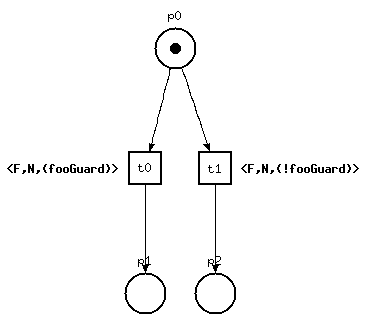
\includegraphics[width=60mm]{Guarda_Como_Decision}
  \caption{Guarda como toma de una decisión.}
  \label{fig:guarda_como_decision}
\end{figure}

\begin{framed}
\textbf{Nota:} Todas las guardas comienzan con valor \mint{java}|false| al
principio de la ejecución del programa.
\end{framed}

\paragraph{Cambiar el valor de una Guarda:} En el siguiente fragmento de código
se muestra cómo cambiar el valor de una guarda \textit{fooGuard}.

\begin{figure}[H]
\centering
\begin{minted}{java}
  // código
  
  // ya fue declarado un PetriMonitor llamado "monitor"
  
  monitor.setGuard("fooGuard", true);
  
  // más código
  
  monitor.setGuard("fooGuard", false);
  
  // más código
\end{minted}
\end{figure}

\subsection{Inicialización del Monitor de Redes de Petri}

Antes de poder operar con el monitor, el usuario debe inicializar algunos
objetos con la información del modelo.

A modo de ejemplo, se asume que existe un archivo PNML que describe la RdP a
utilizar en la dirección ``/path/a/mi/red/de/petri.pnml''. El siguiente
fragmento de código inicializa  el entorno:

\begin{figure}[H]
\centering
\begin{minted}{java}
public void setUp() {
  PetriNetFactory factory = new PetriNetFactory("/path/a/mi/red/de/petri.pnml");
  PetriNet petri = (PlaceTransitionPetriNet) factory.makePetriNet(petriNetType.PT);
  TransitionsPolicy policy = new FirstInLinePolicy();
  PetriMonitor monitor = new PetriMonitor(petri, policy);
  
  // declarar e los hilos de trabajo aquí
  
  // se debe inicializar la RdP antes de poder utilizarla
  petri.initializePetriNet();
  
  // iniciar la ejecución de los hilos de trabajo
  
  // el hilo principal puede realizar otra tarea
  // mientras los hilos de trabajo se ejecutan
  // en este ejemplo, se imprime el marcado de la red cada 5 segundos
  
  while(true){
    try{
      Thread.sleep(5000);
      System.out.println(petri.getCurrentMarking());
    } catch (InterruptedException e){
    }
  }
}
\end{minted}
\end{figure}

\subsection{Disparo de una Transición}

El disparo de una transición se realiza en exclusión mutua dentro del monitor,
es decir de una instancia de la clase \textit{``PetriMonitor''}. La forma de
hacerlo es llamando a alguna de las alternativas del método
\mint{java}|PetriMonitor.fireTransition()|.

Existen dos formas de disparar una transición: mediante el objeto
\textit{Transition} o por nombre de la transición.
En el siguiente ejemplo se muestra la declaración de un hilo que dispara una
transición por cada una de las variantes.

\begin{figure}[H]
\centering
\begin{minted}{java}
  Thread worker = new Thread( new Runnable() {
  
    @Override
    public void run() {
      try {
      
        // sentencias a ejecutar fuera de la exclusión mutua

        // disparo por nombre de transición
        monitor.fireTransition("NombreDeUnaTransicion");

        // otras tareas

        // disparo por objeto Transition
        Transition t0 = petri.getTransition()[0];
        monitor.fireTransition(t0);
      
        // otras tareas
      
        // quizá disparar otra transición de ser necesario

      } catch (IllegalArgumentException | NotInitializedPetriNetException e) {
        // manejar las excepciones
      }
    }
  });
  worker.start();
\end{minted}
\end{figure}

\subsubsection*{Disparos Perennes}
\label{disparos_perennes}
Existe un segundo parámetro para el disparo de una transición: 
\mint{java}|boolean notPerennialFire|. Tiene valor por defecto
\mint{java}|false| e indica si el disparo a realizar es no-perenne.

Si se intenta disparar una transición no sensibilizada de forma perenne, el hilo
que intenta hacer el disparo se bloquea en la cola de condición asociada
(comportamiento por defecto). Por otro lado, si el disparo es no-perenne, el
hilo que intenta hacer el disparo no se bloquea y sale del monitor.

Los disparos no-perenne son útiles cuando el disparo equivale a una acción que
se intenta efectuar únicamente si están dadas las condiciones y no de otra
manera. Un ejemplo de esto es encender una luz; si la luz ya está encendida la
acción no termina, pero el resultado final es el esperado de todas formas.

En el caso del disparo no-perenne de una transición temporal, el hilo
llamador puede bloquearse únicamente si el intento de disparo ocurre antes del
principio del intervalo dinámico de la transición (ver sección
\ref{semantica_tiempo_debil}). Este tipo de bloqueo es temporizado y no requiere
de la activación por medio de otro hilo.

\begin{framed}
\textbf{Nota:} Como el disparo de una transición puede bloquear el hilo que lo
ejecuta, no se recomienda utilizar el hilo principal para realizar disparos
porque puede llevar al bloqueo del programa.
\end{framed}

\begin{framed}
\textbf{Nota:} El disparo explícito de una transición automática es un error
grave, que lleva a que se lance un error
\mint{java}|IllegalTransitionFiringError|.
\end{framed}

\subsection{Política de Transiciones}

Cuando cambia una condición de sensibilización (marcado de la red o valor de
una guarda), algunas transiciones pueden sensibilizarse. Si esto sucede, se
deben disparar las transiciones automáticas sensibilizadas y se debe señalizar a
los hilos que estaban esperando por una transición recientemente sensibilizada.

Si un cambio en las condiciones de sensibilización habilita una sola
transición es trivial cuál transición disparar o cuál hilo señalizar. De otro
modo, la \textit{política} a seguir puede generar o evitar conflictos entre las
transiciones a disparar.
La \textit{política de transiciones} es la que debe decidir qué transición tiene
la mayor prioridad entre el conjunto de todas las transiciones sensibilizadas.

\javapetriconcurrencymonitor incluye dos políticas por defecto. Estas son:
\begin{itemize}
    \item FirstInLinePolicy: Elige la primer transición sensibilizada del
    conjunto dado.
    \item RandomPolicy: Elige una transición de forma aleatoria de entre todas
    las sensibilizadas.
\end{itemize}

Se puede asignar una política de transiciones al monitor de dos formas:

\begin{itemize}
    \item Durante la inicialización, pasando un objeto instancia de
    \textit{TransitionsPolicy} al constructor de \textit{PetriMonitor}.
    \item En tiempo de ejecución, mediante el método\\ {
    \begin{minted}{java}
  PetriMonitor.setTransitionsPolicy(
    TransitionsPolicy _transitionsPolicy)
    \end{minted}
    }
\end{itemize}

\paragraph{Creación de una Política de Transiciones:}
Cualquier instancia de una clase que extienda la clase abstracta
\textit{TransitionsPolicy} puede ser usada como política de transiciones.
La forma de especificar la próxima transición a elegir sobre un conjunto es
implementando el método \mint{java}|public int which(boolean[] enabled)| donde:
\begin{itemize}
    \item El array booleano recibido por parámetro está ordenado por índice de
    las transiciones en la matriz de incidencia, y se corresponde con el orden
    del array de transiciones de \mint{java}|PetriNet.getTransitions()|. Una
    posición con valor \mint{java}|true| indica que la transición cuyo índice
    corresponde con la posición del array, está sensibilizada.
    \item El valor de retorno es el índice de la próxima transición a disparar
    o un valor negativo si no hay transiciones sensibilizadas.
\end{itemize}

En el siguiente ejemplo se muestra cómo definir una política de transiciones
para utilizar con el monitor de RdP. En este caso, se utiliza una clase anónima
de Java y se realiza en el momento de inicialización del monitor:

\begin{figure}[H]
\centering
\begin{minted}{java}
  // código
  
  // se asume que existe un objeto PetriMonitor llamado "petri"
  
  PetriMonitor monitor = new PetriMonitor(petri, TransitionsPolicy(petri) {

    @Override
    public int which(boolean[] enabled) {
      int ret = 0;
      // se debe dar algún valor a "ret"
      // siguiendo el criterio de la política a aplicar
      return ret;
    }

  });
  
  // más código
\end{minted}
\end{figure}

En el próximo ejemplo, se muestra el cuerpo de una clase que implementa una
política estática, definiendo un órden de prioridad de las transiciones mediante sus
nombres:

\begin{figure}[H]
\centering
\begin{minted}{java}
public class OrderedPrioritiesPolicy extends TransitionsPolicy {

    private int[] priorityArray = {
        petri.getTransition("fin_proceso_01").getIndex(),
        petri.getTransition("fin_proceso_02").getIndex(),
        petri.getTransition("comienzo_proceso_01").getIndex(),
        petri.getTransition("comienzo_proceso_02").getIndex()
    };

    public OrderedPrioritiesPolicy(PetriNet _petri){
        super(_petri)
    }
    
    @Override
    public int which(boolean[] enabled) {
        for(int index : priorityArray) {
            if(enabled[index]) {
                return index;
            }
        }
        
        return -1;
    }
}
\end{minted}
\end{figure}

\begin{framed}
\textbf{Nota:} la implementación de una política de transiciones de forma
incorrecta puede llevar a situaciones de conflicto que terminen en la inanición
de uno o más hilos de ejecución.
\end{framed}